%%%%%%%%%%%%%%%%%%%%%%%%%%%%%%%%%%%%%%%%%%%%%%%%%
%%%% LaTeX Problem Set Template
%%%% Konstantin Kashin
%%%% Harvard University
%%%%%%%%%%%%%%%%%%%%%%%%%%%%%%%%%%%%%%%%%%%%%%%%%

\documentclass[10pt,letter]{article}
	% basic article document class
	% use percent signs to make comments to yourself -- they will not show up.

\usepackage{amsmath}
\usepackage{amssymb}
	% packages that allow mathematical formatting

\usepackage{graphicx}
	% package that allows you to include graphics

\usepackage{setspace}
	% package that allows you to change spacing

\onehalfspacing
	% text become 1.5 spaced (can also do \doublespacing; default
        % is single space)

\usepackage{fullpage}
	% package that specifies normal margins


%%%%%%% More advanced packages that support optional functionality in document %%%%%%%%

\usepackage{palatino}
        % package that changes font to Palatino

\usepackage[usenames,dvipsnames]{color}
       % package that allows one to change font color (specifically,
       % 68 colors known to dvips that can be referenced by name)

\usepackage{hyperref}
       % package that allows for hyperlinks in document (useful for
       % cross-referencing figures and tables within document)

%%%%%%%%%%%%%%%%%%%%%%%%%%%%%%%%%%%%%%%%%%%%%%%%%

\begin{document}
	% line of code telling latex that your document is beginning


\title{Problem Set Template}

\author{Your Name Here}

\date{Due Date, 2012}
	% Note: when you omit this command, the current dateis automatically included
 
\maketitle 
	% tells latex to follow your header (e.g., title, author) commands.


\section*{Problem 1}

\paragraph{A)} Answer to Problem 1(A) here. To illustrate how to use
the \verb/eqnarray*/ and the in-line math environments, I have included a sample response
(to a problem from a causal inference class in the Statistics Department at Harvard).
\\
\\
{\color{Orchid}
We can show that regression on just the treatment
indicator is identical to the average treatment effect obtained from
Neyman. Let us specify a linear regression as: $Y_i^{obs} = \beta_0 +
\beta_1 \cdot W_i + \varepsilon_i$, where $W_i$ is the treatment
indicator for unit $i$ and $\varepsilon_i \sim \mathcal{N}(0, \sigma^2)$.
\\
\\
Then, we know that minimizing the sum of squared residuals over the
coefficients yields: \\
\\
 $\hat{\tau}_{OLS} = \dfrac{\sum (W_i-\bar{W}) (Y_i^{obs} -
   \bar{Y}^{obs})}{\sum (W_i-\bar{W})^2}$
\\
\\
Let's work with the numerator first and rewrite it: \\
\begin{small}
\begin{eqnarray*}
\sum (W_i-\bar{W}) (Y_i^{obs} -
   \bar{Y}^{obs}) &=& \sum_{i: W_i =0}  -\bar{W} (Y_i^{obs} -
   \bar{Y}^{obs}) + \sum_{i: W_i =1} (1-\bar{W}) (Y_i^{obs} -
   \bar{Y}^{obs}) \\
& = & -\bar{W} \sum_{i: W_i =0} (Y_i^{obs} -
   \bar{Y}^{obs}) + (1-\bar{W}) \sum_{i: W_i =1} (Y_i^{obs} -
   \bar{Y}^{obs}) \\
& = & -\bar{W} \sum_{i: W_i =0} (Y_i^{obs}) + \bar{W} N_C
\bar{Y}^{obs} +  (1-\bar{W}) \sum_{i: W_i =1} (Y_i^{obs})  -
(1-\bar{W}) N_T \bar{Y}^{obs}  \\
& = & -\bar{W} \sum_{i: W_i =0} (Y_i^{obs}) +  (1-\bar{W}) \sum_{i: W_i =1} (Y_i^{obs})  -
N_T \bar{Y}^{obs} +\bar{W} N_T \bar{Y}^{obs} +    \bar{W} N_C
\bar{Y}^{obs}   \\
& = & -\bar{W} \sum_{i: W_i =0} (Y_i^{obs}) +  (1-\bar{W}) \sum_{i: W_i =1} (Y_i^{obs})  -
N_T \bar{Y}^{obs} +\bar{W} N \bar{Y}^{obs}  \\
& = & -\dfrac{N_T}{N} \sum_{i: W_i =0} (Y_i^{obs}) +
(1-\dfrac{N_T}{N}) \sum_{i: W_i =1} (Y_i^{obs})  - N_T \bar{Y}^{obs}
+\dfrac{N_T}{N} \cdot N \bar{Y}^{obs}  \\
& = & -\dfrac{N_T}{N} \sum_{i: W_i =0} (Y_i^{obs}) +
(1-\dfrac{N_T}{N}) \sum_{i: W_i =1} (Y_i^{obs}) \\
& = & \dfrac{N_C}{N} \sum_{i: W_i =1} (Y_i^{obs}) -\dfrac{N_T}{N} \sum_{i:
  W_i =0} (Y_i^{obs})  \\
\end{eqnarray*}
\end{small}}
\\
\fbox{{\color{BrickRed} We could put the final answer in a box like this, and/or change
  the color to make it stand out.}}

\subparagraph{i)} Answer to Problem 1(A)(i) here.


\subparagraph{ii)} Answer to Problem 1(A)(ii) here.

\subparagraph{iii)} Answer to Problem 1(A)(iii) here.

\paragraph{B)} Answer to Problem 1(B) here.
\\
\\
Example of typesetting a table. Note that I omitted the \verb/table/
environment because I didn't want the captioning or the table as a
float (but generally, this is recommended when dealing with many
tables since they are automatically numbered).\\
{\color{Orchid}
\\
%\begin{table}
\begin{tabular}{|c|c|c|c|}
\hline
 \textbf{Subclass} & \textbf{Estimated Propensity Score Bounds} & \textbf{Number Treated Units} &
 \textbf{Number Control Units} \\
\hline
 1 & [0,0.00104] & 1 & 278 \\
\hline
2&  (0.00104, 0.00469]  & 1 & 277  \\
\hline
3&  (0.00469, 0.0184]  & 4 & 275  \\
\hline
4&  (0.0184,0.1289]  & 10 & 268  \\
\hline
5&  (0.1289,1]  & 169 & 110  \\
\hline
\end{tabular}
%\end{table}
}

\subparagraph{i)} Answer to Problem 1(B)(i) here.

\subparagraph{ii)} Answer to Problem 1(B)(ii) here.

\subparagraph{iii)} Answer to Problem 1(B)(iii) here.

\paragraph{C)} Answer to Problem 1(C) here.
\\
\\
Example of typesetting Figure \ref{fig:myfigure} using the \verb/figure/ environment. Note how due to figure size,
\LaTeX\phantom{a}automatically pushes it onto the next page, despite
the fact that we have specified \verb/h!/ as an option telling
\LaTeX\phantom{a}to place the float exactly here. Omitting \verb/h!/
as an option would lead to the figure being positioned at the end of
the document, which may be preferable in some cases. Note that I am
using the \verb/hyperref/ package to provide hyperlink support and
cross-referencing between where I mention ``Figure 1'' in the text
above and where the actual graphic is
positioned in the text (this is a more advanced function and is purely optional).
\begin{figure}[h!]
  \centering
  \caption{Distributions of Estimated Propensity Scores for Original Sample}
  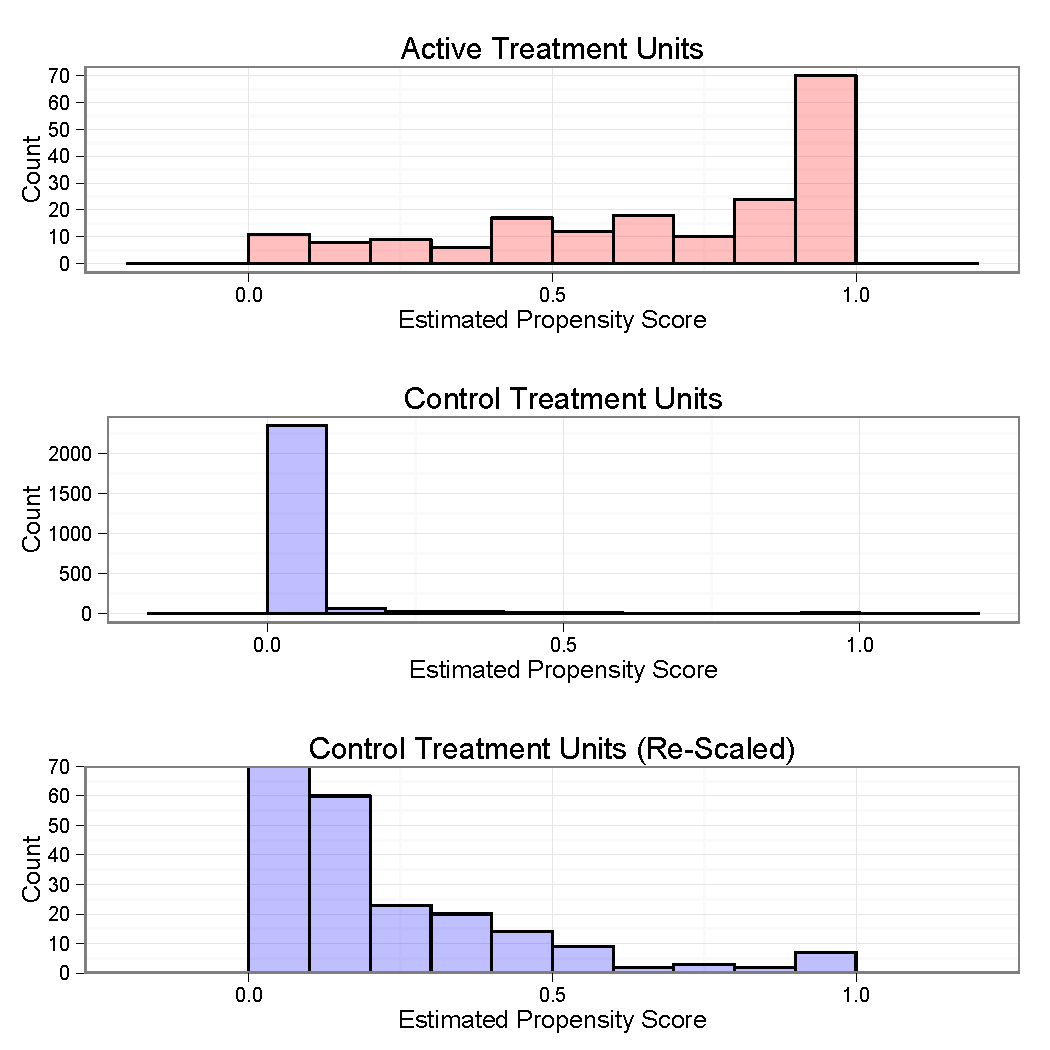
\includegraphics[width=0.5\textwidth]{propscore-ex.pdf}
\label{fig:myfigure}
\end{figure}

\paragraph{D)} Answer to Problem 1(D) here.

\paragraph{E)} Answer to Problem 1(E) here.


\section*{Problem 2}

\paragraph{A)} Answer to Problem 2(A) here.

\paragraph{B)} Answer to Problem 2(B) here.


\section*{Problem 3} Answer to Problem 3 here.


\section*{Problem 4}

\paragraph{A)} Answer to Problem 4(A) here.

\paragraph{B)}  Answer to Problem 4(B) here.


\end{document}
	% line of code telling latex that your document is ending. If you leave this out, you'll get an error
